\chapter{Interacciones}
\section{Introduccion}
\begin{flushleft}El diagrama de secuencia es un tipo de diagrama de interaccion cuyo objetivo es describir el comportamiento dinamico del sistema de informacion haciendo enfasis en la secuencia de los mensajes intercambiados por los objetos.
	\\
	En este caso se va a representar cada caso de uso planteado anteriormente en un diagrama de
	secuencia, y cada caso de uso con sus respectivos escenarios primario, secundario y excepcional que tambien fueron expresados anteriormente.
	\\
	Los diagramas fueron elaborados con ayuda de la herramienta Coloso y estan basados en las descripciones de los casos de uso propuestos en la seccion anterior.\end{flushleft}

\begin{flushleft}\end{flushleft}

\newpage
\section{Diagramas de Secuencia}
% \subsection{Elementos de UML}
\subsubsection{CASO DE USO: Servicio de Parqueo de Vehiculo}
\begin{center}
	El siguiente diagrama inicia con el usuario accediendo al programa en esta fase este ya ha iniciado sesión, por el primer mensaje se procede a mostrarle el mapa al usuario y una vez seleccione un parqueadero en el mapa el cual causa que se envíe un mensaje a la parte lógica con el código del parqueadero seleccionado, bien ahora la parte logica envia el mensaje a la base de datos solicitando información del parqueadero. Ahora el usuario confirma el parqueadero lo cual de igual manera envia un mensaje a la lógica para acceder y modificar la base de datos respecto al parqueadero.
\end{center}
\begin{table}[H]
	\begin{tabular}{|c|l|l}
		\cline{1-2}
		\multicolumn{2}{|c|}{Escenario Primario:}                                                                      & \multicolumn{1}{r}{} \\ \cline{1-2}
		\multicolumn{2}{|c|}{\begin{tabular}[c]{@{}c@{}}{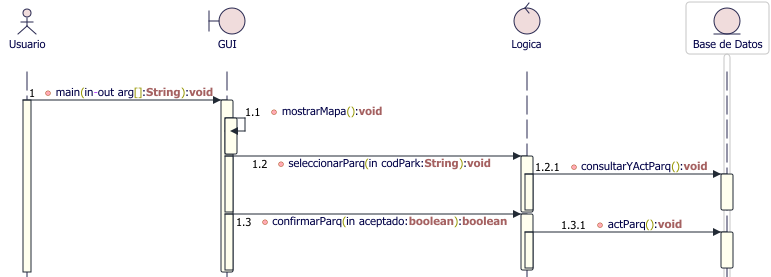
\includegraphics[width=1.15\linewidth]{imgs/DiagramaSecuancia-CasosdeUso/Imagenes/caso1} } \\ \end{tabular}} &                      \\ \cline{1-2}
	\end{tabular}
\end{table}
\begin{center}
	Ahora para el caso secundario necesitamos un retorno para que el usuario conozca el estado del parqueadero seleccionado, el cual siguiendo el paso de mensajes que consulta la información del parqueadero almacenada en la base de datos, este retornara un 
	dato que se tomará como booleano para por medio de un mensaje cíclico muestre al usuario si está disponible este parqueadero.
\end{center}
\begin{table}[H]
	\begin{tabular}{|c|l|l}
		\cline{1-2}
		\multicolumn{2}{|c|}{Escenario Secundario:}                                                                      & \multicolumn{1}{r}{} \\ \cline{1-2}
		\multicolumn{2}{|c|}{\begin{tabular}[c]{@{}c@{}}{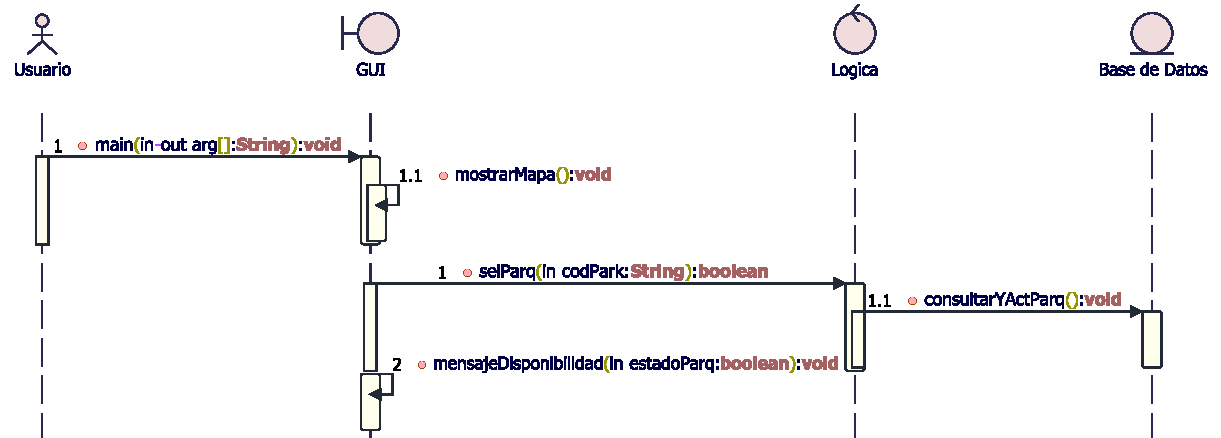
\includegraphics[width=1.15\linewidth]{imgs/DiagramaSecuancia-CasosdeUso/Imagenes/caso1segundario} } \\ \end{tabular}} &                      \\ \cline{1-2}
	\end{tabular}
\end{table}
\begin{center}
	En el caso excepcional se parte de que antes de mostrar el mapa al usuario este se obtiene por un mensaje enviado a la lógica para obtenerlo de la base de datos el cual obtendrá el estado de los parqueaderos ubicados en el mapa para que el usuario sepa cuales están disponibles.
\end{center}
\begin{table}[H]
	\begin{tabular}{|c|l|l}
		\cline{1-2}
		\multicolumn{2}{|c|}{Escenario Excepcional:}                                                                      & \multicolumn{1}{r}{} \\ \cline{1-2}
		\multicolumn{2}{|c|}{\begin{tabular}[c]{@{}c@{}}{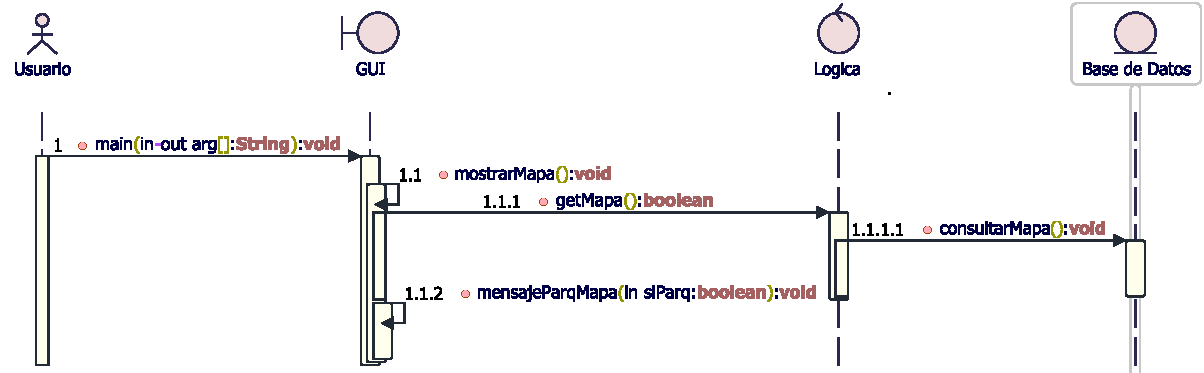
\includegraphics[width=1.15\linewidth]{imgs/DiagramaSecuancia-CasosdeUso/Imagenes/caso1excep} } \\ \end{tabular}} &                      \\ \cline{1-2}
	\end{tabular}
\end{table}


\newpage

\subsubsection{CASO DE USO: Parqueo por tipo de Vehiculo}
\begin{center}
	Este parte del mismo punto que el caso anterior por ende el paso de mensajes es el mismo, ahora bien teniendo en cuenta que el usuario necesita saber si el parqueadero seleccionado es compatible con el tipo de vehículo esta información se obtendrá de la base de datos la cual me verificará por medio de un retorno booleano si es compatible lo cual se mostrará al usuario por medio de un mensaje cíclico.
\end{center}
\begin{table}[H]
	\begin{tabular}{|c|l|l}
		\cline{1-2}
		\multicolumn{2}{|c|}{Escenario Primario:}                                                                      & \multicolumn{1}{r}{} \\ \cline{1-2}
		\multicolumn{2}{|c|}{\begin{tabular}[c]{@{}c@{}}{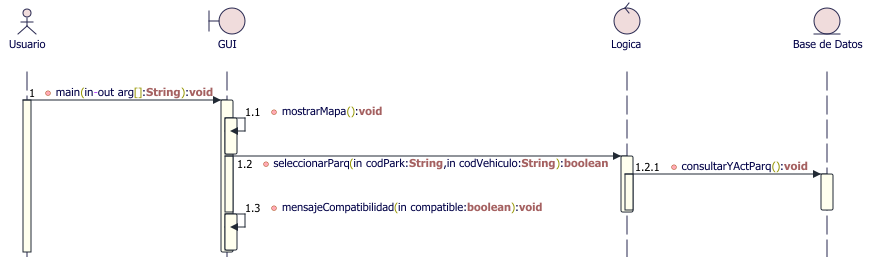
\includegraphics[width=1.15\linewidth]{imgs/DiagramaSecuancia-CasosdeUso/Imagenes/caso2} } \\ \end{tabular}} &                      \\ \cline{1-2}
	\end{tabular}
\end{table}
\begin{center}
	Teniendo en cuenta la secuencia anterior el paso de mensajes no es muy diferente lo que se agrega para tratar este caso es por medio de un mensaje cíclico que el usuario verá en forma de ventana emergente que impide que se pueda registrar en el parqueadero en caso de que este no sea compatible.
\end{center}
\begin{table}[H]
	\begin{tabular}{|c|l|l}
		\cline{1-2}
		\multicolumn{2}{|c|}{Escenario Secundario:}                                                                      & \multicolumn{1}{r}{} \\ \cline{1-2}
		\multicolumn{2}{|c|}{\begin{tabular}[c]{@{}c@{}}{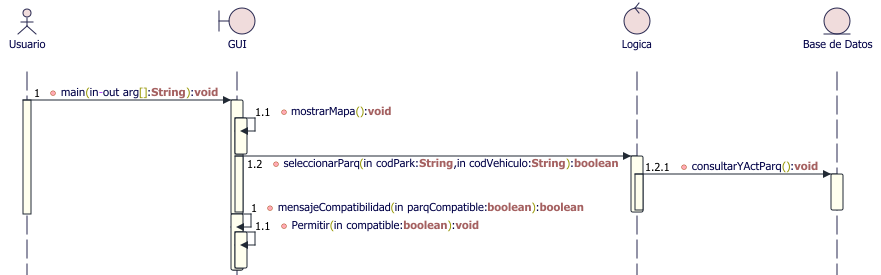
\includegraphics[width=1.15\linewidth]{imgs/DiagramaSecuancia-CasosdeUso/Imagenes/caso2segundario} } \\ \end{tabular}} &                      \\ \cline{1-2}
	\end{tabular}
\end{table}
\begin{center}
	Ahora bien para este caso se debe tratar desde que se muestra el mapa al usuario, este antes de mostrar el mapa de la base de datos pasa por un filtro que se da por el paso de mensajes el cual envia un codigo que es el tipo de vehiculo del usuario para determinar su compatibilidad, y en caso de que retorne 0 parqueaderos que sean compatibles se enviara un mensaje cíclico el cual le notificará al usuario que no se encuentran parqueaderos compatibles en el área.
\end{center}
\begin{table}[H]
	\begin{tabular}{|c|l|l}
		\cline{1-2}
		\multicolumn{2}{|c|}{Escenario Excepcional:}                                                                      & \multicolumn{1}{r}{} \\ \cline{1-2}
		\multicolumn{2}{|c|}{\begin{tabular}[c]{@{}c@{}}{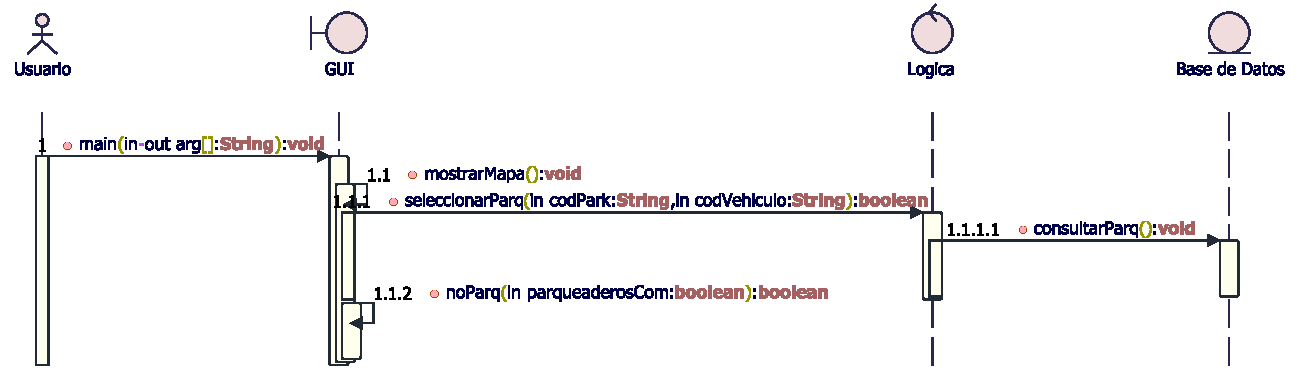
\includegraphics[width=1.15\linewidth]{imgs/DiagramaSecuancia-CasosdeUso/Imagenes/caso2excep} } \\ \end{tabular}} &                      \\ \cline{1-2}
	\end{tabular}
\end{table}

\newpage


\subsubsection{CASO DE USO: Consulta de Servicios}

\begin{center}
	En el Escenario Primario del caso de uso de Consultas de Servicios, se plantea una precondicion en la cual el usuario ya debe haber adquirido un servicio de parqueo, por lo que podra desplegar un menu de servicios desde la Interfaz del programa, y podra consultar cualquiera de estos servicios que se encuentren disponibles para el parqueo que ya ha sido adquirido.
\end{center}

\begin{table}[H]
	\begin{tabular}{|c|l|l}
		\cline{1-2}
		\multicolumn{2}{|c|}{Escenario Primario:}                                                                      & \multicolumn{1}{r}{} \\ \cline{1-2}
		\multicolumn{2}{|c|}{\begin{tabular}[c]{@{}c@{}}{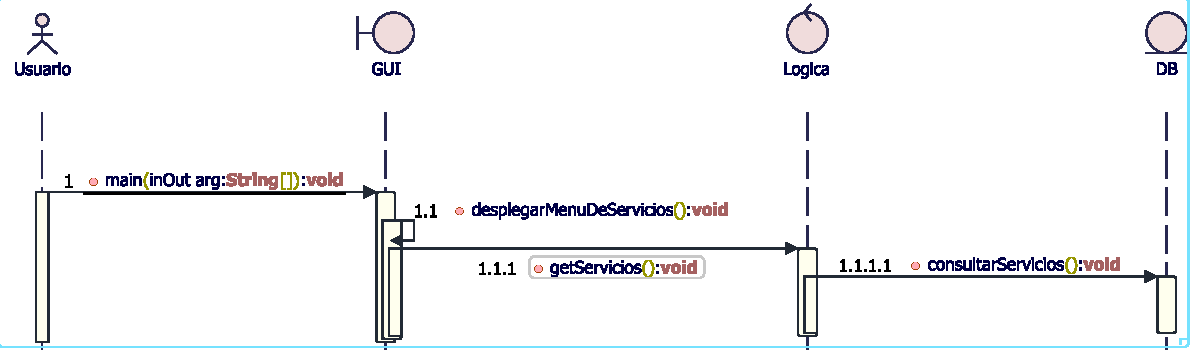
\includegraphics[width=1.15\linewidth]{imgs/DiagramaSecuancia-CasosdeUso/ConsultasdeServicios/ConsultasdeServicio-primario} } \\ \end{tabular}} &                      \\ \cline{1-2}
	\end{tabular}
\end{table}
\begin{center}
En el Escenario Secundario, se plantea la posibilidad de que el usuario selecciono un servicio que es posible que el espacio que adquirio antes ofrecia, pero en este momento ya no se encuentra disponible, como una renovacion de alquiler un dia que el parqueo ya se encuentra ocupado.
\end{center}


\begin{table}[H]
	\begin{tabular}{|c|l|l}
		\cline{1-2}
		\multicolumn{2}{|c|}{Escenario Secundario:}                                                                      & \multicolumn{1}{r}{} \\ \cline{1-2}
		\multicolumn{2}{|c|}{\begin{tabular}[c]{@{}c@{}}{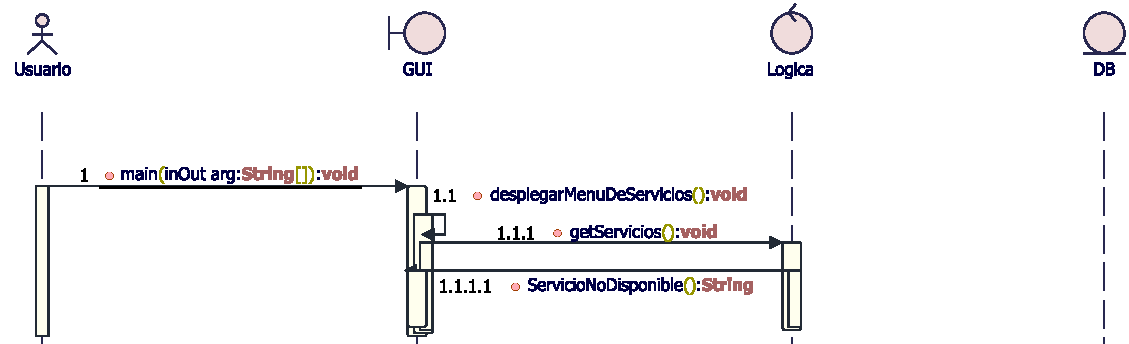
\includegraphics[width=1.15\linewidth]{imgs/DiagramaSecuancia-CasosdeUso/ConsultasdeServicios/ConsultasdeServicio-segundario} } \\ \end{tabular}} &                      \\ \cline{1-2}
	\end{tabular}
\end{table}
\begin{center}
	En el Escenario Excepcional, es posible que un usuario ya registrado y logeado, haya podido seleccionar la opcion de consulta de servicios sin previamente haber adquirido un servicio de parqueo.
\end{center}
\begin{table}[H]
	\begin{tabular}{|c|l|l}
		\cline{1-2}
		\multicolumn{2}{|c|}{Escenario Excepcional:}                                                                      & \multicolumn{1}{r}{} \\ \cline{1-2}
		\multicolumn{2}{|c|}{\begin{tabular}[c]{@{}c@{}}{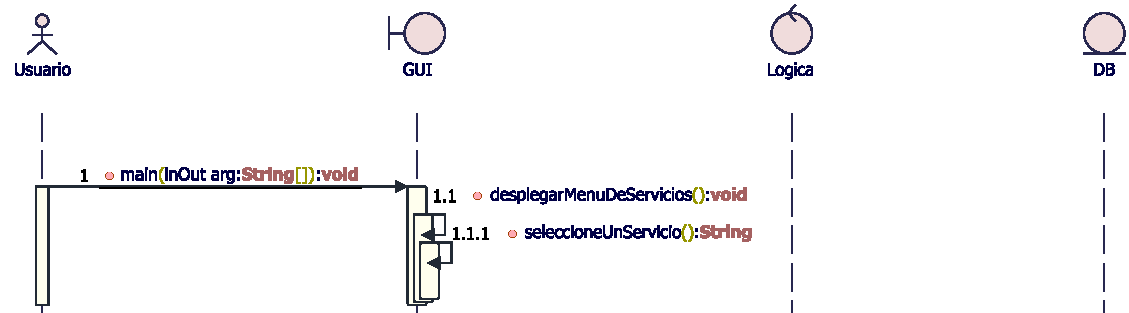
\includegraphics[width=1.15\linewidth]{imgs/DiagramaSecuancia-CasosdeUso/ConsultasdeServicios/ConsultasdeServicio-excepcional} } \\ \end{tabular}} &                      \\ \cline{1-2}
	\end{tabular}
\end{table}

\newpage
\subsubsection{CASO DE USO: Geolocalizacion}
\begin{center}
	En el Escenario Primario del caso de uso de Geolocalizacion, se tiene en cuenta que el usuario previamente se ha registrado y logeado, y ha concedido los permisos necesarios para poder desplegar la interfaz de geolocalizacion, interfaz en la que el usuario podra solicitar la ubicacion en tiempo real de un espacio que quiera alquilar, y la API de google maps se lo muestre.
\end{center}
\begin{table}[H]
	\begin{tabular}{|c|l|l}
		\cline{1-2}
		\multicolumn{2}{|c|}{Escenario Primario:}                                                                      & \multicolumn{1}{r}{} \\ \cline{1-2}
		\multicolumn{2}{|c|}{\begin{tabular}[c]{@{}c@{}}{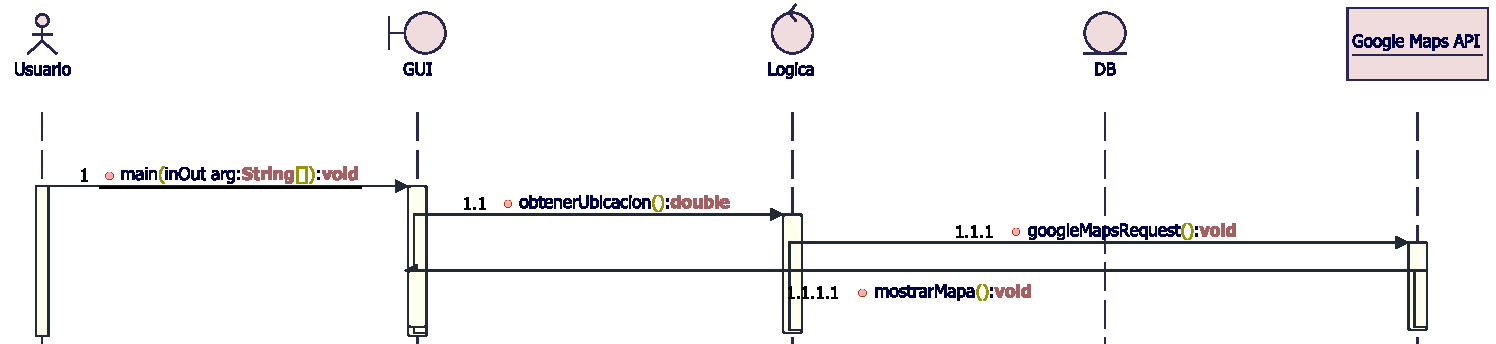
\includegraphics[width=1.15\linewidth]{imgs/DiagramaSecuancia-CasosdeUso/Geolocalizacion/Geolocalizacion-primario} } \\ \end{tabular}} &                      \\ \cline{1-2}
	\end{tabular}
\end{table}
\begin{center}
	En el Escenario Secundario se plantea una situacion en la que un servicio especifico seleccionado por el usuario no se encuentra disponible en la zona solicitada.
\end{center}
\begin{table}[H]
	\begin{tabular}{|c|l|l}
		\cline{1-2}
		\multicolumn{2}{|c|}{Escenario Secundario:}                                                                      & \multicolumn{1}{r}{} \\ \cline{1-2}
		\multicolumn{2}{|c|}{\begin{tabular}[c]{@{}c@{}}{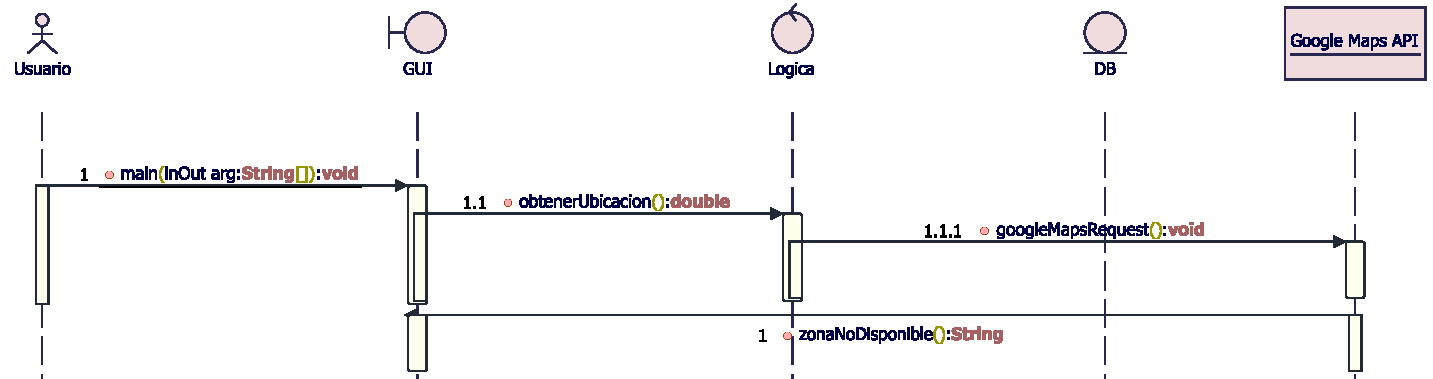
\includegraphics[width=1.15\linewidth]{imgs/DiagramaSecuancia-CasosdeUso/Geolocalizacion/Geolocalizacion-secundario} } \\ \end{tabular}} &                      \\ \cline{1-2}
	\end{tabular}
\end{table}
\begin{center}
	En el Escenario Excepcional es posible que el usuario no haya concedido los permisos necesarios para el correcto funcionamiento de la API de google maps
\end{center}
\begin{table}[H]
	\begin{tabular}{|c|l|l}
		\cline{1-2}
		\multicolumn{2}{|c|}{Escenario Excepcional:}                                                                      & \multicolumn{1}{r}{} \\ \cline{1-2}
		\multicolumn{2}{|c|}{\begin{tabular}[c]{@{}c@{}}{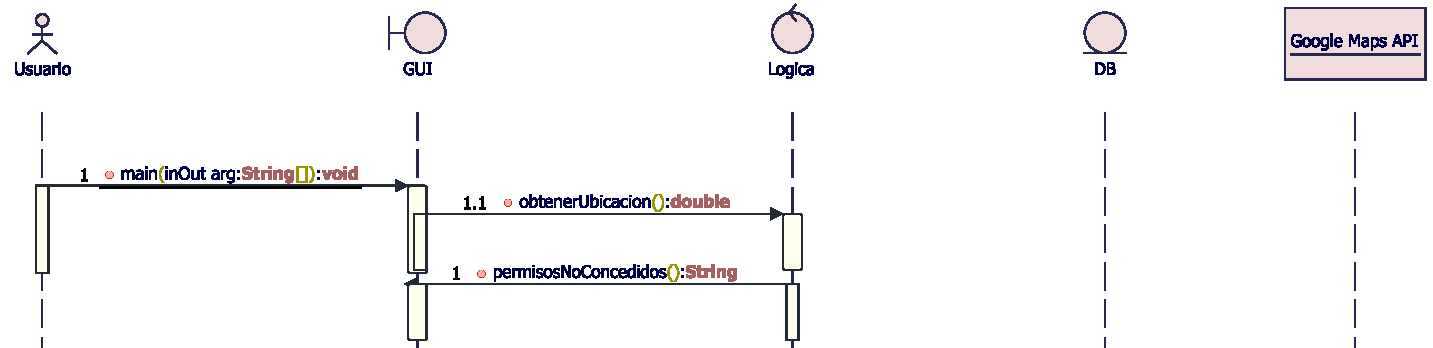
\includegraphics[width=1.15\linewidth]{imgs/DiagramaSecuancia-CasosdeUso/Geolocalizacion/Geolocalizacion-excepcional} } \\ \end{tabular}} &                      \\ \cline{1-2}
	\end{tabular}
\end{table}

\newpage


%--------------------------DIAGRAMAS DE COMUNICACIONES----------------------


\newpage
 \section{Diagramas de Comunicación}
 \subsubsection{CASO DE USO: Servicio de Parqueo de Vehiculo}
 \begin{table}[H]
 	\begin{tabular}{|c|l|l}
 		\cline{1-2}
 		\multicolumn{2}{|c|}{Escenario Primario:}                                                                      & \multicolumn{1}{r}{} \\ \cline{1-2}
 		\multicolumn{2}{|c|}{\begin{tabular}[c]{@{}c@{}}{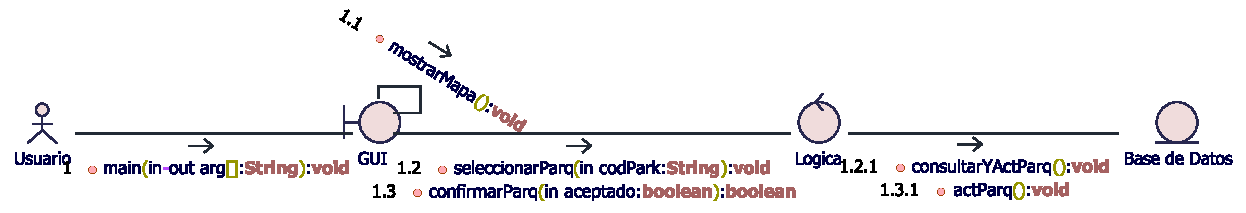
\includegraphics[width=1.15\linewidth]{imgs/DiagramaSecuancia-CasosdeUso/Imagenes/caso1com} } \\ \end{tabular}} &                      \\ \cline{1-2}
 	\end{tabular}
 \end{table}
 
 \begin{table}[H]
 	\begin{tabular}{|c|l|l}
 		\cline{1-2}
 		\multicolumn{2}{|c|}{Escenario Secundario:}                                                                      & \multicolumn{1}{r}{} \\ \cline{1-2}
 		\multicolumn{2}{|c|}{\begin{tabular}[c]{@{}c@{}}{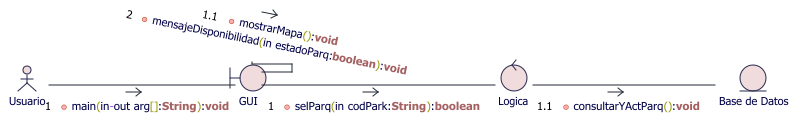
\includegraphics[width=1.15\linewidth]{imgs/DiagramaSecuancia-CasosdeUso/Imagenes/caso1segundariocom} } \\ \end{tabular}} &                      \\ \cline{1-2}
 	\end{tabular}
 \end{table}
 
 \begin{table}[H]
 	\begin{tabular}{|c|l|l}
 		\cline{1-2}
 		\multicolumn{2}{|c|}{Escenario Excepcional:}                                                                      & \multicolumn{1}{r}{} \\ \cline{1-2}
 		\multicolumn{2}{|c|}{\begin{tabular}[c]{@{}c@{}}{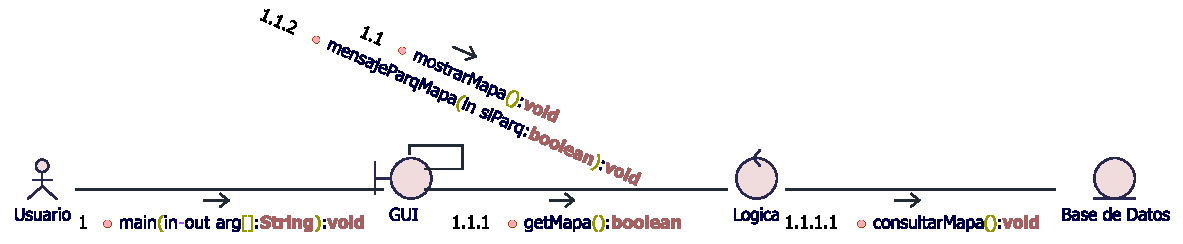
\includegraphics[width=1.15\linewidth]{imgs/DiagramaSecuancia-CasosdeUso/Imagenes/caso1excepcom} } \\ \end{tabular}} &                      \\ \cline{1-2}
 	\end{tabular}
 \end{table}
 \newpage
 
 \subsubsection{CASO DE USO: Parqueo por tipo de Vehiculo}
 \begin{table}[H]
 	\begin{tabular}{|c|l|l}
 		\cline{1-2}
 		\multicolumn{2}{|c|}{Escenario Primario:}                                                                      & \multicolumn{1}{r}{} \\ \cline{1-2}
 		\multicolumn{2}{|c|}{\begin{tabular}[c]{@{}c@{}}{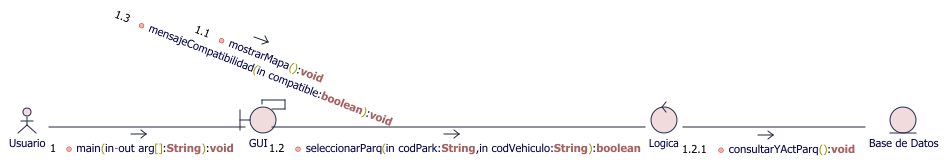
\includegraphics[width=1.15\linewidth]{imgs/DiagramaSecuancia-CasosdeUso/Imagenes/caso2com} } \\ \end{tabular}} &                      \\ \cline{1-2}
 	\end{tabular}
 \end{table}
 
 \begin{table}[H]
 	\begin{tabular}{|c|l|l}
 		\cline{1-2}
 		\multicolumn{2}{|c|}{Escenario Secundario:}                                                                      & \multicolumn{1}{r}{} \\ \cline{1-2}
 		\multicolumn{2}{|c|}{\begin{tabular}[c]{@{}c@{}}{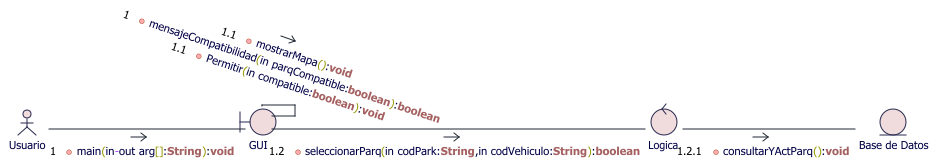
\includegraphics[width=1.15\linewidth]{imgs/DiagramaSecuancia-CasosdeUso/Imagenes/caso2segundariocom} } \\ \end{tabular}} &                      \\ \cline{1-2}
 	\end{tabular}
 \end{table}
 
 \begin{table}[H]
 	\begin{tabular}{|c|l|l}
 		\cline{1-2}
 		\multicolumn{2}{|c|}{Escenario Excepcional:}                                                                      & \multicolumn{1}{r}{} \\ \cline{1-2}
 		\multicolumn{2}{|c|}{\begin{tabular}[c]{@{}c@{}}{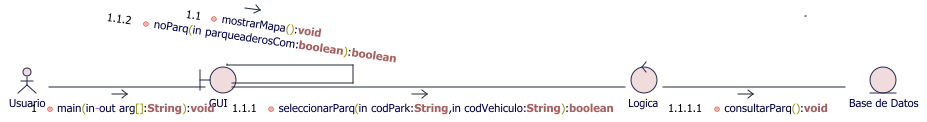
\includegraphics[width=1.15\linewidth]{imgs/DiagramaSecuancia-CasosdeUso/Imagenes/caso2excepcom} } \\ \end{tabular}} &                      \\ \cline{1-2}
 	\end{tabular}
 \end{table}
 \newpage
 
\subsubsection{CASO DE USO: Consulta de Servicios}

% \newpage
\begin{table}[H]
	\begin{tabular}{|c|l|l}
		\cline{1-2}
		\multicolumn{2}{|c|}{Escenario Primario:}                                                                      & \multicolumn{1}{r}{} \\ \cline{1-2}
		\multicolumn{2}{|c|}{\begin{tabular}[c]{@{}c@{}}{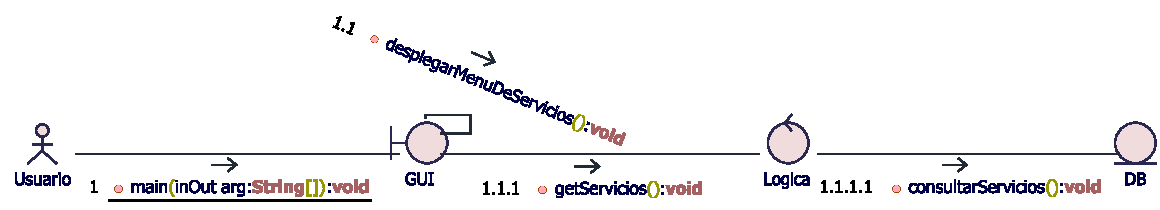
\includegraphics[width=1.15\linewidth]{imgs/DiagramaSecuancia-CasosdeUso/ConsultasdeServicios/ConsultadeServicioPrimarioComunicacion} } \\ \end{tabular}} &                      \\ \cline{1-2}
	\end{tabular}
\end{table}

\begin{table}[H]
	\begin{tabular}{|c|l|l}
		\cline{1-2}
		\multicolumn{2}{|c|}{Escenario Secundario:}                                                                      & \multicolumn{1}{r}{} \\ \cline{1-2}
		\multicolumn{2}{|c|}{\begin{tabular}[c]{@{}c@{}}{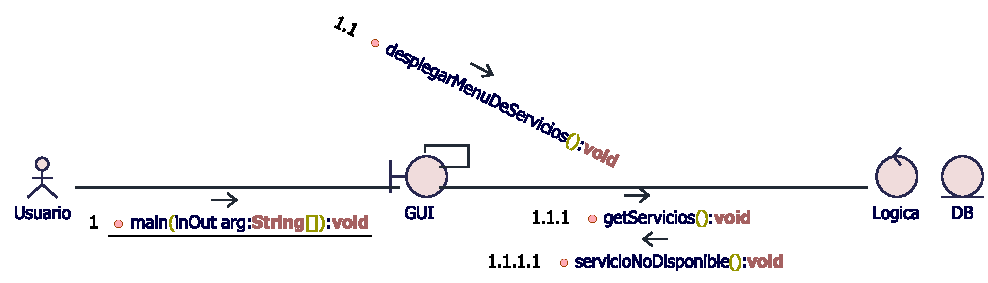
\includegraphics[width=1.15\linewidth]{imgs/DiagramaSecuancia-CasosdeUso/ConsultasdeServicios/ConsultadeServicioSecundarioComunicacion} } \\ \end{tabular}} &                      \\ \cline{1-2}
	\end{tabular}
\end{table}

\begin{table}[H]
	\begin{tabular}{|c|l|l}
		\cline{1-2}
		\multicolumn{2}{|c|}{Escenario Excepcional:}                                                                      & \multicolumn{1}{r}{} \\ \cline{1-2}
		\multicolumn{2}{|c|}{\begin{tabular}[c]{@{}c@{}}{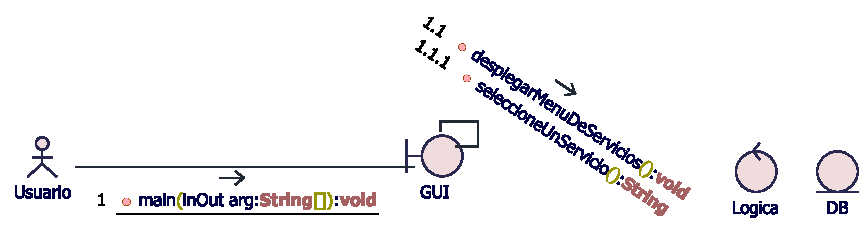
\includegraphics[width=1.15\linewidth]{imgs/DiagramaSecuancia-CasosdeUso/ConsultasdeServicios/ConsultadeServicioExcepcionalComunicacion} } \\ \end{tabular}} &                      \\ \cline{1-2}
	\end{tabular}
\end{table}

\newpage
\subsubsection{CASO DE USO: Geolocalizacion}

\begin{table}[H]
	\begin{tabular}{|c|l|l}
		\cline{1-2}
		\multicolumn{2}{|c|}{Escenario Primario:}                                                                      & \multicolumn{1}{r}{} \\ \cline{1-2}
		\multicolumn{2}{|c|}{\begin{tabular}[c]{@{}c@{}}{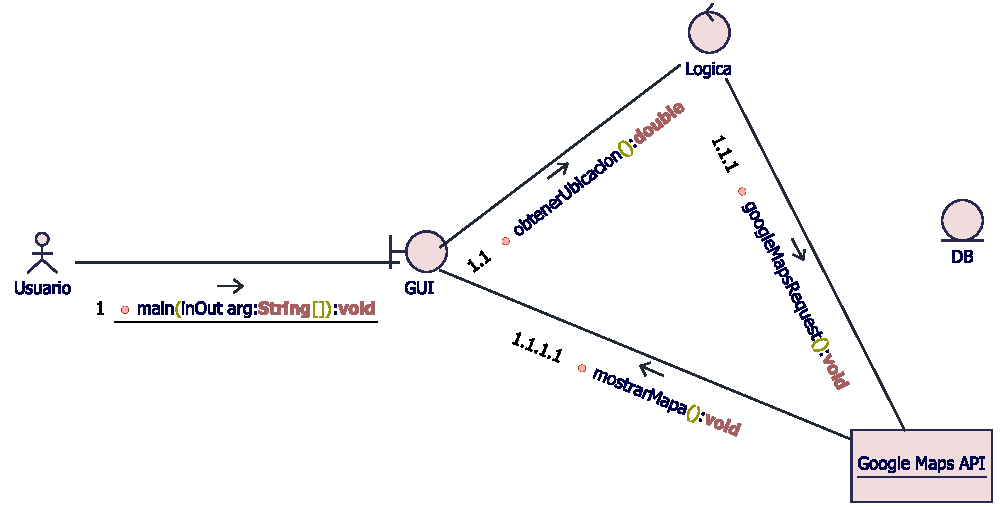
\includegraphics[width=1.15\linewidth]{imgs/DiagramaSecuancia-CasosdeUso/Geolocalizacion/GeolocalizacionPrimarioComunicacion} } \\ \end{tabular}} &                      \\ \cline{1-2}
	\end{tabular}
\end{table}

\begin{table}[H]
	\begin{tabular}{|c|l|l}
		\cline{1-2}
		\multicolumn{2}{|c|}{Escenario Secundario:}                                                                      & \multicolumn{1}{r}{} \\ \cline{1-2}
		\multicolumn{2}{|c|}{\begin{tabular}[c]{@{}c@{}}{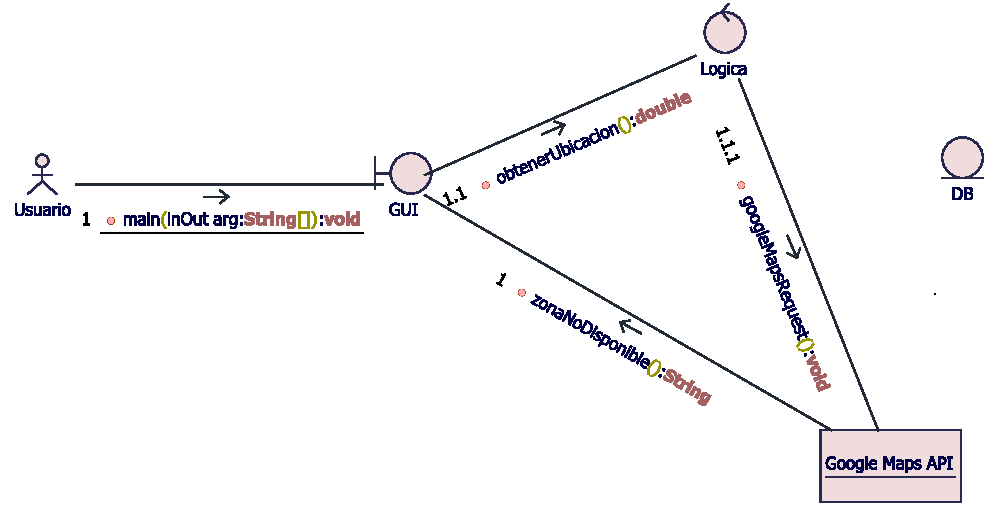
\includegraphics[width=1.15\linewidth]{imgs/DiagramaSecuancia-CasosdeUso/Geolocalizacion/GeolocalizacionSecundarioComunicacion} } \\ \end{tabular}} &                      \\ \cline{1-2}
	\end{tabular}
\end{table}

\begin{table}[H]
	\begin{tabular}{|c|l|l}
		\cline{1-2}
		\multicolumn{2}{|c|}{Escenario Excepcional:}                                                                      & \multicolumn{1}{r}{} \\ \cline{1-2}
		\multicolumn{2}{|c|}{\begin{tabular}[c]{@{}c@{}}{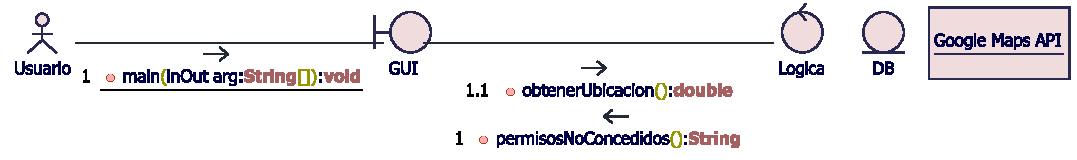
\includegraphics[width=1.15\linewidth]{imgs/DiagramaSecuancia-CasosdeUso/Geolocalizacion/GeolocalizacionExcepcionalComunicacion} } \\ \end{tabular}} &                      \\ \cline{1-2}
	\end{tabular}
\end{table}
\newpage